% !TeX spellcheck = it_IT

\section{Problemi di ottimizzazione}

Sono un caso particolare dei problemi come precedentemente definiti.\\

Un \textbf{problema di ottimizzazione} $\pi$: 
\begin{enumerate}
	\item \textbf{Input} $I_\pi \subseteq 2^\ast$
	
	\item Una \textbf{funzione} $Amm_\pi: \, I_\pi \rightarrow 2^{2^\ast} \setminus \{\emptyset\}$ \textbf{mappa} ogni \textbf{input} in un \textbf{insieme di soluzioni ammissibili}
	
	\item $c_\pi: 2^\ast \times 2^\ast \rightarrow \mathbb{N}$, $\forall x \in I_\pi$, $\forall y \in Amm_\pi (y)$, $c_\pi (x,y)$, ovvero un costo/guadagno, \textbf{funzione obiettivo}
	
	\item $T_\pi \in \{\max, \min\}$: "tipo del problema", voglio massimizzare o minimizzare il mio costo/guadagno
\end{enumerate}

\paragraph{Esempio:} Max-Sat
\begin{itemize}
	\item input: formule logiche in forma CNF, esempio:
	$$ (x_7 \vee x_2) \wedge (x_4 \vee \neg x_5 \vee \neg x_7) \wedge (x_9 \neg x_2) $$
	
	\item Le soluzioni ammissibili per una data formula $\varphi$ sono tutti gli assegnamenti delle variabili di di $\varphi$, quindi per l'esempio tutte le $2^5$ possibili combinazioni di assegnamenti delle $5$ variabili
	
	\item $c_\pi (\varphi, ass)$: il costo per ogni formula con un dato assegnamento è il numero di clausole rese vere dall'assegnamento
	
	\item $T_\pi = \max$: problema di massimizzazione, voglio un assegnamento che massimizzi il numero di clausole soddisfatte
\end{itemize}

Ovviamente non si può avere un algoritmo polinomiale che risolve questo problema in quanto sarebbe equivalente al CNF-SAT, avere il massimo numero di clausole soddisfacibili vorrebbe dire anche sapere se la formula è soddisfacibile.\\

\newpage

\subsection{Problema di decisione associato} 

Ad \textbf{ogni problema di ottimizzazione} $\pi$ \textbf{si può associare un problema di decisione} $\hat{\pi}$:
\begin{itemize}
	\item $I_{\hat{\pi}} = (x, k)$, $x \in I_\pi$, $k \in \mathbb{N}$.\\
	\item La risposta per l'input $(x,k)$ è sì iff $\exists y \in Amm_\pi (x)$ esiste una soluzione ammissibile tale che $c_\pi (x,y) \geq k$ per i problemi di massimizzazione, oppure $c_\pi (x,y) \leq k$ per problemi di minimizzazione (rientro nel costo $k$?).\\
\end{itemize}

Sostanzialmente, "trovare il minimo" diventa "esiste una soluzione con costo minore di $k$?".\\

\paragraph{Esempio:} per $\hat{\text{Max-Sat}}$
\begin{itemize}
	\item $I_{\hat{\text{Max-Sat}}} = \{ (\varphi, k) | \, \varphi$ formula CNF e $k \in \mathbb{N} \}$.\\
	\item $(\varphi, k)$ è \textit{sì} iff $\exists$ assegnamento che rende vere almeno $k$ clausole di $\varphi$.\\
\end{itemize}

\newpage

\subsection{Classe di complessità $\mathcal{PO}$}
Si definisce $\mathcal{PO}$ l'insieme dei problemi di ottimizzazione $\pi$ tali che $\pi$ è risolvibile in tempo polinomiale
$$ \mathcal{PO} = \{\pi \text{ problemi di ott. } | \, \pi \text{ risolvibile in t polinomiale } \}$$

\addcontentsline{toc}{subsubsection}{\protect\numberline{}Teorema}
\paragraph{Teorema:} Se $\pi \in \mathcal{PO}$, allora il suo problema di decisione associato sta in $\mathcal{P}$, i.e. $\hat{\pi} \in \mathcal{P}$.\\

\paragraph{Corollario:} Al contrario, se il problema di decisione associato $\hat{\pi}$ è $\mathcal{NP}c$, allora il problema non può essere risolto in tempo polinomiale $\pi \notin \mathcal{PO}$ (assumendo $\mathcal{P} \neq \mathcal{NP}$).\\

Esempio di problemi in PO: problemi di programmazione lineare. Mentre restringere il campo a solamente a soluzioni intere fa diventare il problema $\mathcal{NP}c$.\\

\newpage

\subsection{Rapporto di prestazione} 

Verranno trattati principalmente problemi che rientrano in $\mathcal{NP}c$, quindi non saranno risolvibili in modo esatto, ma solamente in modo approssimato. Ma come si quantifica l'approssimazione? \\

Dato un p.o. $\pi$, chiamiamo $\opt_\pi (x)$ il \textbf{valore ottimo della funzione obiettivo su input} $x$.\\
Dato un \textbf{algoritmo approssimato} $A$ (in input prende un possibile input ed in output fornisce una soluzione ammissibile, ma non necessariamente ottima) per $\pi$, definisco il \textbf{rapporto di approssimazione} 
$$ R_\pi (x) = \max \left\{\frac{c_\pi (x,y)}{opt_pi(x)}, \frac{opt_\pi (x)}{c_\pi (x,y)} \right\} $$
Il $\max$ serve a prendere un valore sempre $\geq 1$, sia per problemi di minimizzazione che massimizzazione, in modo da avere una definizione unica.\\

Si dice che $A$ è una \textbf{$\alpha$-approssimazione} per $\pi$ iff 
$$ \forall x \in I_\pi : \, R_\pi (x) \leq \alpha $$
Per ogni input $R_\pi (x)$ è minore o uguale di $\alpha$, sostanzialmente comunque vada quell'algoritmo non può essere peggio di $\alpha$ sul problema $\pi$. Ovviamente con $\alpha = 1$ l'algoritmo è esatto ed il problema sta in $\mathcal{PO}$.\\

\newpage

\subsection{Altre classi}
Si hanno altre possibili classi di problemi: 
\begin{itemize}
	\item Fuori da $\mathcal{PO}$ ($\mathcal{PO} \subset$), ci sono le classi \textbf{$n$-APX}, quindi $2$-APX ad esempio sono gli algoritmi che risolvono con $\alpha$ fino a 2 volte, 3 fino a 3 volte, ...; sostanzialmente classi sempre più grandi fino ad avere approssimazioni arbitrariamente grandi.\\
	
	\item \textbf{APX}: problemi risolvibili a meno di una costante di approssimazione di qualche tipo arbitrariamente grande, ma costante. Sempre algoritmi polinomiali, ma approssimati.\\
	
	\item Poi \textbf{$\log n$-APX}: approssimati ma l'approssimazione dipende anche dalla dimensione dell'input, fuori da APX (APX $\subset$).\\
	
	\item Tutte queste classi sono contenute in $\mathcal{NPO}$, ovvero l'equivalente di ottimizzazione di $\mathcal{NP}$.\\
	
	\item esistono anche problemi $\mathcal{NPO}$-completi $\mathcal{NPO}c$, ed interseca tutti i sottoinsiemi fin'ora (tranne $\mathcal{PO}$ ovviamente).\\
	
	\item \textbf{PTAS} (polinomial time approximation scheme), (appena fuori $\mathcal{PO}$): problemi approssimabili "quanto voglio", quindi posso decidere il tasso di approssimazione ma il tempo peggiora di conseguenza, anche in modo anche esponenziale.\\
	
	\item \textbf{FPTAS} (fully PTAS): dentro PTAS, fuori $\mathcal{PO}$, come PTAS, ma il tempo peggiora esclusivamente in modo polinomiale.\\
\end{itemize}

Dovrei mettere un disegnino con i cerchietti ma non ho assolutamente voglia, si capisce anche così dai (spero).\\

\newpage

% End of L2

\subsection{Problema di MaxMatching} 
Caratteristiche del problema: 
\begin{itemize}
	\item \textbf{Input:} un \textbf{grafo non orientato} $G = (V, E)$ e bipartito (due gruppi di nodi, i nodi all'interno di un gruppo non hanno collegamenti tra loro)
	\item \textbf{Soluzioni ammissibili:} chiamate \textbf{matching}, insieme $M$, una selezione di lati per cui nessun vertice incide su $>1$ lato, scegliere lati in modo da coprire il maggior numero di vertici possibili senza coprire nessun vertice più di una volta
	
	\item \textbf{Funzione obiettivo:} numero di lati scelti, ovvero \textbf{cardinalità di} $M$
	
	\item \textbf{Tipo:} problema di \textbf{massimizzazione} $= \max$, massimizzare il numero di vertici coperti
\end{itemize}

In questo caso la \textbf{soluzione ottima} si può trovare in \textbf{tempo polinomiale}, questo problema rientra in $\mathcal{PO}$. \\

\paragraph{Algoritmo del cammino aumentante:} un cammino aumentante viene definito su un grafo su cui è già presente un matching, anche parziale (solo in realtà, altrimenti non aumento nulla). Un \textbf{vertice} viene definito "\textbf{esposto}" quando su quel vertice \textbf{non incide nessun lato del matching}. \\

Un \textbf{augmenting path} è un \textbf{cammino} che \textbf{parte e arriva su un vertice esposto} ed \textbf{alterna lati} "liberi" (\textbf{non nel matching}) \textbf{e lati} "presi" (\textbf{nel matching}). Sequenza di lati alternata che inizia e termina su un vertice esposto. Partendo da vertici esposti il primo lato è per forza non preso.\\

Sapendo che c'è un cammino aumentante, è possibile scambiare i lati presi e non presi, si può fare uno \textbf{switch} sul cammino aumentante trovato. Partendo ed arrivando su nodi esposti per il cammino, \textbf{facendo lo switch} ci sarà sempre un \textbf{lato in più} "preso" \textbf{nel matching} e di conseguenza due nodi in più.\\

Se \textbf{ho un cammino aumentante posso migliorare il matching}, quindi quest'ultimo non è ottimo. Per migliorare il matching basta trovare un cammino aumentante, di conseguenza se lo trovo posso migliorare il matching, altrimenti il matching è massimo.\\

\paragraph{Lemma:} se \textbf{esiste un cammino aumentante} per il matching $M$, allora $M$ \textbf{non è massimo}.\\

\paragraph{Lemma 2:} se $M$ \textbf{non è massimo} allora \textbf{esiste un cammino aumentante}.\\

\begin{proof}
	Sia $M'$ un altro matching con $|M'| > |M|$ ($M$ non è massimo, ne esiste uno con cardinalità maggiore). Di conseguenza, considerando gli insiemi dei lati presi da ognuno dei matching, abbiamo tre zone tra i due insiemi: 
	\begin{itemize}
		\item lati in comune $M \cap M'$
		\item lati solo nell'insieme più piccolo $M \setminus M'$
		\item lati solo nell'insieme più grande $M' \setminus M$
	\end{itemize}
	
	Prendendo la differenza simmetrica tra i due
	$$ M \Delta M' = (M \setminus M') \cup (M' \setminus M)$$
	
	\textbf{Considerazione:} Nessun vertice può avere più di 2 lati coincidenti in $M \Delta M'$; se in ogni insieme possono avere un solo lato incidente ed ho due insiemi non possono essere più di 2 lati totali, il grado di ogni vertice sarà $\leq 2$, inoltre se ne ha 2 uno viene da un insieme ed uno dall'altro. \\ 
	Di conseguenza sul grafo generato dai lati in $M \Delta M'$ esiste $\exists$ almeno un cammino, composto da lati presi alternativamente uno da un insieme ed uno dall'altro, non possono essere di fila altrimenti vorrebbe dire che un vertice è stato considerato due volte all'interno dello stesso matching.\\
	Sapendo che $|M'| > |M|$ ci deve essere almeno un cammino che inizia e finisce con un lato di $M' \setminus M$ dato che sono di più e non può essere un ciclo (altrimenti sarebbero due lati dello stesso matching sullo stesso vertice). \\
	
	Essendo questo cammino alternanza di lati presenti in $M \setminus M'$ e lati in $M' \setminus M$ questo vuol dire che è un cammino aumentante per $M$.\\
\end{proof}

\newpage

%Questo è a prescindere dalle cose prima, serve per spiegare la roba dopo
\subsection*{Visite di grafi}
\addcontentsline{toc}{subsection}{\protect\numberline{}Visite di grafi}
Un po' estemporaneo ma serve spiegarlo.\\

Con "visite di grafi" si intende \textbf{metodi sistematici per "scoprire" un grafo}. Durante una visita i \textbf{nodi} possono rientrare in \textbf{3 categorie}:
\begin{itemize}
	\item sconosciuti, bianchi $W$ 
	\item conosciuti ma non visitati, grigi $G$, detti anche frontiera di visita
	\item visitati, neri $B$
\end{itemize}

La visita funziona iniziando \textbf{mettendo nella frontiera un solo nodo}, chiamato seed della visita. 
$$ F \leftarrow \{x_{seed}\}$$

Quindi in questo momento il nodo seme è grigio, tutti gli altri bianchi.
\begin{algorithm}
	\caption{VisitaGrafo ($Graph$)}
	\begin{algorithmic}
		\STATE $\forall x$ $c(x) \leftarrow W$
		\STATE $F \leftarrow \{x_{seed}\}$
		\STATE $c (_{seed}) \leftarrow G$
		\WHILE{$F \neq \emptyset$}
		\STATE $x \leftarrow $ pick$(F)$
		\STATE visit $x$
		\STATE $c(x) \leftarrow B$
		\FOR{$i \in $ neighbor$(x)$}
		\IF{$c(y) == W$}
		\STATE $F \leftarrow F \cup \{y\}$
		\STATE $c(y) = G$
		\ENDIF
		\ENDFOR
		\ENDWHILE
	\end{algorithmic}
\end{algorithm}

\newpage

Quando la frontiera è non-vuota, prendo un nodo dalla frontiera e visito questo nodo (qualunque cosa significhi). Coloro questo nodo di nero. Guardo tutti i vicini di questo nodo e:
\begin{itemize}
	\item se sono neri, già visitati, oppure grigi, già conosciuti, li lascio lì
	\item se sono bianchi li metto nella frontiera e li coloro di grigio
\end{itemize}

Per un grafo orientato l'unica cosa che cambia è scegliere se visitare i vicini uscenti o entranti (collegati con archi uscenti o entranti).\\

Se il \textbf{grafo è connesso} questo \textbf{garantisce di visitare ogni vertice una volta sola}. Se non è connesso verrà visitata solo la parte connessa del seme, per continuare serve un altro seed.\\

In base a \textbf{come viene scelto il nodo da prendere nella frontiera cambia il tipo di visita}, ad esempio con uno stack viene una DFS, con una coda viene una BFS, ma in generale, in base a come viene implementata la scelta del nodo si ha un tipo di visita diversa.\\

\newpage

\subsubsection{Trovare un cammino aumentante}
Un cammino aumentante deve \textbf{iniziare e terminare su un nodo esposto}, partendo da un grafico ed un matching. \\

Come \textbf{trovo nodi esposti}? faccio, partendo da ogni nodo \textbf{una BFS che alterna lati all'interno di} $M$ \textbf{e lati al di fuori di} $M$.\\

Se \textbf{una BFS} ad un certo punto \textbf{trova altri nodi esposti} allora abbiamo un \textbf{cammino aumentante}, altrimenti si passa alle BFS sul prossimo nodo, se \textbf{non viene trovato nessun altro nodo esposto} in nessun nodo allora \textbf{non ci sono cammini aumentanti}.\\

\begin{algorithm}
	\caption{FindAugmenting(G,M)}
	\begin{algorithmic}
		\STATE $X \leftarrow$ vertici esposti in $M$
		\FOR{all $x \in X$}
		\STATE  BFS$(x)$ con alternanza di lati $\notin M$ e $\in M$
		\ENDFOR
	\end{algorithmic}
\end{algorithm}

\paragraph{Tempo:} la BFS richiede tempo proporzionale al numero di lati $O(N \cdot M)$, una BFS per ogni vertice esposto, quindi al massimo $O(n^2)$. Quante volte dobbiamo eseguire FindAugmenting? al limite $n/2$, quindi $O(n/2 \cdot n^2) \subset O(n^3)$.\\

\addcontentsline{toc}{subsubsection}{\protect\numberline{}Teorema}
\paragraph{Teorema:} BipartiteMaxMatching $\in \mathcal{PO}$.\\

\paragraph{Corollario:} il problema di decisione PerfectMatching (il grafo ammette un matching massimale) è $\in \mathcal{P}$.\\

\newpage

Perché la BFS non funziona su grafi non bipartiti?
\begin{center}
	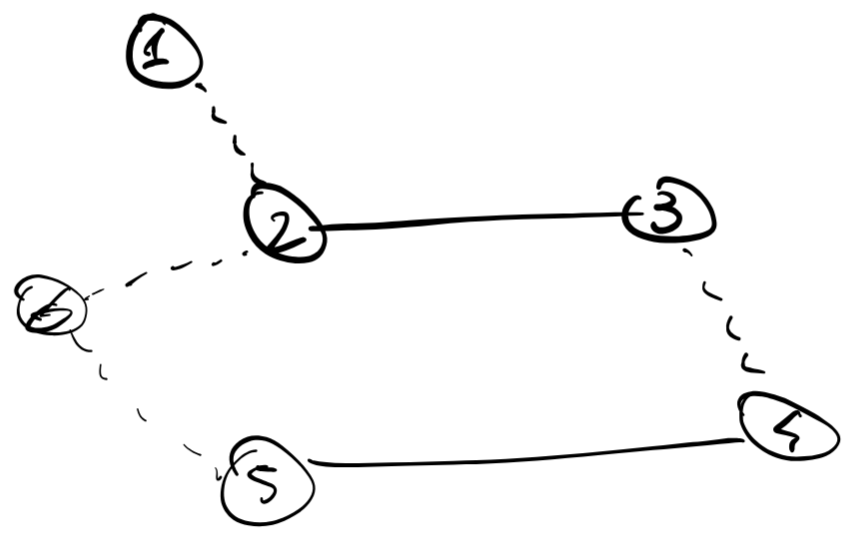
\includegraphics[width=0.8\columnwidth]{img/bipartito1}
\end{center}
Partendo da qualsiasi nodo esposto in questo grafo non si possono trovare cammini aumentanti (prova a farci la BFS alternata se non mi credi, stronzo (non ho voglia di scriverla)).\\

\newpage

\section{Tecniche greedy}

\subsection{Problema di LoadBalancing}
Non ammette una soluzione polinomiale ottima $\in \mathcal{NPO}$.\\

Problema in cui si ha \textbf{un numero di task} di una certa \textbf{durata} e bisogna \textbf{dividerli su varie macchine} in modo da avere la massima \textbf{durata di ogni macchina al minimo possibile}:
\begin{itemize}
	\item \textbf{Input:} $m > 0$ numero di macchine, $n>0$ numero di task, $(t_i)_{i \in n}$, durate dei task, $t_i > 0$
	
	\item \textbf{Output:} $\alpha: n \rightarrow m$, assegnare ogni task ad una macchina. Il carico della macchina $j$ è definito come 
	$$ L_j := \sum_{i: \alpha (i) = j} t_i$$
	La somma di tutte le durate dei task assegnati a quella macchina. Il carico massimo è
	$$ L := \max_j \{L_j\}$$ 
	il valore più alto di una singola macchina
	
	\item \textbf{Funzione obiettivo:} $L$
	
	\item \textbf{Tipo:} problema di minimizzazione $\min$, devo minimizzare il costo della macchina con il costo più alto
\end{itemize}

\addcontentsline{toc}{subsubsection}{\protect\numberline{}Teorema}
\paragraph{Teorema:} LoadBalancing $\in \mathcal{NPO}c$.\\

\textbf{Definizione di $\mathcal{NPO}c$:} un problema di ottimizzazione $\pi$ è $\in \mathcal{NPO}c$ iff $\pi \in \mathcal{NPO}$ e $\hat{\pi} \in \mathcal{NP}c$, il problema di decisione associato è $\mathcal{NP}c$.\\

\newpage

\subsubsection{Algoritmo greedy per LoadBalancing}

Fornisce una \textbf{soluzione approssimata}. Sostanzialmente l'algoritmo consiste nel \textbf{prendere i task} ed associarli sempre alla macchina più "scarica", con la attuale durata complessiva delle task minore.\\

Chiamando $A_i$ l'insieme dei \textbf{task associati alla macchina} $i$.\\

All'inizio sia task associati che carichi totali partono a zero. Si itera su tutti i task, si sceglie la macchina con il carico minore e si aggiunge alla sua lista di task il task $j$ considerato (ed il carico relativo).\\
Ovviamente è polinomiale: $O(n)$ per cercare tra i task e $O(m)$ per cercare le macchine, quindi il totale $O(nm)$

\begin{algorithm}
	\caption{GreedyLoadBalancing$(n, m)$}
	\begin{algorithmic}
		\STATE $A_i \leftarrow \emptyset$ $\forall i \in n$
		\STATE $L_i \leftarrow \emptyset$ $\forall i \in n$
		\FOR{$j =  0, \, ... \, , m-1$}
		\STATE $\overline{i} \leftarrow \arg \min_i L_i$
		\STATE $A_{\overline{i}} \leftarrow A_{\overline{i}} \cup \{j\}$
		\STATE $L_{\overline{i}} \rightarrow L_{\overline{i}} + t_j$
		\ENDFOR
	\end{algorithmic}
\end{algorithm}

\addcontentsline{toc}{subsubsection}{\protect\numberline{}Teorema}
\paragraph{Teorema:} GreedyBalance è una 2-Approssimazione per Loadbalancing

\begin{proof}
	Chiamando $L^\ast$ il valore della funzione obiettivo della soluzione ottima. \\
	
	\textbf{Osservazione 1:} posso dire che 
	$$ L^\ast \geq \frac{1}{m} \sum_{j} t_j $$
	
	Ovviamente se potessi dividere il totale di tutti i task in modo perfetto su $m$ macchine otterrei una soluzione ideale (1/m del tempo totale per ogni macchina), quindi la soluzione ottima deve essere per forza $\geq$ di questa divisione.\\
	
	\textbf{Osservazione 2 }
	$$ L^\ast \geq \max_j t_j $$
	Il compito più grande qualcuno lo deve fare, quindi il tempo massimo non può essere inferiore al tempo del task più lungo.\\
	
	Sia $\hat{i}$ tale che $L_{\hat{i}} = L$ e sia $\hat{j}$ l'ultimo compito che le è stato assegnato.\\
	
	Prima di assegnare alla macchina $\hat{i}$ l'ultimo carico, questa doveva essere quella con il carico minore di tutte
	$$ L_{\hat{i}} - t_{\hat{j}} \leq L_i ' \;\;\;\;\; \forall i \in m $$
	$$ m (L_{\hat{i}} - t_{\hat{j}}) \leq \sum_i L_i = \sum_j t_j $$
	$$ \implies L_{\hat{i}} - t_{\hat{i}} \leq \frac{1}{m} \sum_j t_j \leq L^\ast $$
	L'ultima parte della disequazione possiamo aggiungerla essendo la stessa cosa della osservazione 1.
	
	$$ L = L_{\hat{i}} = L_{\hat{i}} - t_{\hat{j}} + t_{\hat{j}} \geq 2 \cdot L^\ast $$
	Per la osservazione 2, posso far vedere che $t_{\hat{j}}$ è $\leq L^\ast$, quindi il totale è tutto minore di $2 \cdot L^\ast$. Di conseguenza possiamo evincere il rapporto di approssimazione
	$$ \frac{L}{L^\ast} \leq 2 $$
	
	L'algoritmo quindi è 2-Approssimato.
\end{proof}

\newpage

% da invertire sopra la frazione, scritto sbagliato

\paragraph{Dimostrazione di tightness:} questa dimostrazione serve a stabilire che $L/L^\ast$ è davvero 2, ovvero che \textbf{il bound non può diminuire ulteriormente} e quel fattore di approssimazione dipende intrinsecamente dall'algoritmo e non da qualche errore nella dimostrazione.\\

\addcontentsline{toc}{subsubsection}{\protect\numberline{}Teorema}
\paragraph{Teorema:} per ogni $\epsilon > 0$, esiste un input per il problema LoadBalancing tale che GreedyLoadBalancing produce un output con 
$$ 2 - \epsilon \leq \frac{L}{L^\ast} \leq 2$$
(ovvero schiaccio quanto voglio il bound).\\

Dobbiamo \textbf{costruire un input} che fa "andare male" l'algoritmo:
\begin{itemize}
	\item numero di macchine $m > 1/ \epsilon$
	\item numero di task $n = m(m-1)+1$
	\item ci sono $m(m-1)$ task lunghi $1$ e $1$ task lungo $m$, presentati in quest'ordine
\end{itemize}

I primi $m$ verranno dati ciascuno ad una macchina, e si ripete $m-1$ volte. Alla fine di questi tutte le macchine hanno lo stesso carico.\\
Poi arriva big task che verrà messo sulla macchina meno carica (sono tutte uguali, quindi una a caso praticamente).\\

Di conseguenza la funzione obiettivo finale sarà:
$$ L = m - 1 + m = 2m - 1 $$

Non sapendo che alla fine arriva il taskone non possiamo prepararci al suo arrivo. La soluzione ottima sarebbe dare il Titanic ad una macchina e dividere gli altri $m(m-1)$ alle altre macchine; alla fine tutte le macchine avranno lo stesso carico, quindi è sicuramente la soluzione ottima, con valore:
$$ L = m $$

Il rapporto di prestazione nel primo caso diventa:
$$ \frac{L}{L^\ast} = \frac{2m-1}{m} = 2 - \frac{1}{m} $$

Essendo un \textbf{algoritmo greedy}, \textbf{l'ordine} dei task è \textbf{importante} ed in questo caso è la differenza tra un input ottimale ed il peggiore.\\

Comunque, magari gli input reali non sono così male, questo algoritmo su input reali potrebbe avere un tasso di approssimazione più basso, potrebbero essere input più favorevoli rispetto alle casistiche considerate in questo modo.\\

\subsubsection{SortedGreedyBalance}
Sempre sul problema di LoadBalancing, sempre stesso input e output dell'algoritmo precedente.\\

L'algoritmo funziona \textbf{ordinando} in ordine \textbf{decrescente i task} e poi \textbf{chiamando l'algoritmo greedy}:

\begin{algorithm}
	\caption{SortedGreedyBalance$(n, m)$}
	\begin{algorithmic}
		\STATE Sort $t_i$ in Non-increasing order
		\item Run GreedyLoadBalancing$(n,m)$
	\end{algorithmic}
\end{algorithm}

Ma è davvero meglio? \\

\addcontentsline{toc}{subsubsection}{\protect\numberline{}Teorema}
\paragraph{Teorema:} SortedGreedyBalance produce una $\frac{3}{2}$-Approssimazione

\begin{proof}
	\textbf{Osservazione 1}: se $n<m$, la soluzione prodotta è ottima (tutti i task a macchine distinte, meglio di così non si può).\\
	
	Da qui in poi viene considerato $n>m$ (almeno una macchina deve avere 2 task assegnati).\\
	
	\textbf{Osservazione 2}: $L^\ast \geq 2 \cdot t_m$. Considerando i task
	$$ t_0 \geq t_1 \geq \, ... \, \geq t_m \geq t_{m+1} \geq \, ... \, \geq t_{n-1} $$
	Almeno una macchina dovrà avere 2 task, uno dai primi $m$ task ed uno dai restanti.\\
	
	\newpage
	
	Sia $\hat{i}$ tale che $L_{\hat{i}} = L$:
	\begin{itemize}
		\item Se $\hat{i}$ ha un task solo, la soluzione è ottima
		\item Se $\hat{i}$ ha più di un compito. Sia $\hat{j}$ l'ultimo compito (ovvero l'indice del task) assegnato a $\hat{i}$
		\item Sicuramente $\hat{j} \geq m$ in quanto i primi $m$ task sono sicuramente dati a macchine distinte (non può esserci una macchina meno carica di una vuota)
	\end{itemize}
	Quindi 
	$$ L = L_{\hat{i}} = \left(L_{\hat{i}} - t_{\hat{j}}\right) + t_{\hat{j}} $$  
	Di conseguenza, sapendo che
	$$ t_{\hat{j}} \leq t_m \leq \frac{1}{2} L^\ast $$
	Possiamo dire
	$$
	\begin{array}{c c}
		\left(L_{\hat{i}} - t_{\hat{j}}\right)  & \leq L^\ast \\
		t_{\hat{j}} & \leq t_{\hat{j}}
	\end{array}
	\implies
	\left(L_{\hat{i}} - t_{\hat{j}}\right) + t_{\hat{j}}  \leq L^\ast + \frac{1}{2} L^\ast = \frac{3}{2} L^\ast
	$$
	In conclusione
	$$ L = L_{\hat{i}} \leq \frac{3}{2}L^\ast $$
	
\end{proof}

Ci vorrebbe una dimostrazione di tightness, ma questa analisi non è tight, si può dimostrare che l'algoritmo in realtà è una $\frac{4}{3}$-Approssimazione (dimostrazione di \href{https://www.jstor.org/stable/pdf/2099572.pdf}{Graham 1969}).\\

Hochbaum-Shmoys 1988 hanno dimostrato che in realtà LoadBalancing apparitene $\in PTAS$, ovvero si può approssimare con una precisione $\epsilon$ qualunque, e scala esponenzialmente il tempo necessario per l'approssimazione, quindi si sa anche che $\notin FPTAS$.\\

\newpage

\subsection{Problema della selezione dei centri CenterSelection}
Avendo vari posti dove smistare pacchi e $n$ soldi per costruire un numero limitato di magazzini, bisogna decidere dove piazzarli. Una volta piazzati tutti gli altri centri di smistamento si rivolgono al magazzino più vicino. Si creano delle celle di Varanoi (Check nome) attorno ai magazzini sostanzialmente. Di conseguenza c'è una distanza massima che un centro di smistamento deve coprire per arrivare al magazzino, ovvero un raggio di copertura, tra tutte le soluzioni si vuole minimizzare questo raggio.\\

Hai dei \textbf{punti in uno spazio metrico} e si vogliono \textbf{scegliere} $k$ \textbf{punti} in questo spazio in modo che il \textbf{raggio di copertura} per tutti sia il \textbf{minore possibile}.\\

\paragraph{Spazio metrico:} un'insieme con una funzione distanza $(\Omega, d)$ 
$$d: \, \Omega  \times \Omega \rightarrow \mathbb{R}^+$$

Con le seguenti proprietà:
\begin{itemize}
	\item $d(x,y) = d(y,x)$ (simmetria)
	\item $d(x,y) = 0$ iff $x=y$
	\item $d(x,y) \leq d(x,z) + d(z,y)$ (disuguaglianza triangolare)
\end{itemize}
L'input per la selezione dei centri sarà immerso in uno spazio metrico.\\

Definizioni: nel mio insieme di punti, qual'è il punto scelto (magazzino) più vicino?
$$ dist(x,A) := \min_{y \in A} d(x,y) $$

$$ \forall s \in S \;\;\; \delta_c (s) := dist(s,C)$$

$$ \rho_c := \max_{s \in S} \delta_c (s) $$

\newpage

\paragraph{Definizione del problema:} fissiamo uno spazio metrico $(\Omega, d)$
\begin{itemize}
	\item \textbf{Input:} un \textbf{insieme} $S \subseteq \Omega$ di $n$ \textbf{punti immersi in uno spazio metrico} fissato ed un \textbf{budget} $k>0$
	
	\item \textbf{Soluzione accettabile:} è un \textbf{sottoinsieme} $C \subseteq S$ con $|C| \leq k$ ($\leq k$ punti nello spazio)
	
	\item \textbf{Funzione obiettivo:} $\rho_c$
	
	\item \textbf{Tipo:} $\min$
\end{itemize}
Vogliamo minimizzare il massimo dei percorsi.\\

\subsubsection{Algoritmo CenterSelectionPlus} 
Facciamo finta di avere in input un parametro che non avremo. Stesso input del problema, ma aggiungiamo 
$$ r \in \mathbb{R}^+ $$

\begin{algorithm}
	\caption{CenterSelectionPlus$(S, k)$}
	\begin{algorithmic}
		\STATE $C \leftarrow \emptyset$
		\WHILE{$S \neq \emptyset$}
		\STATE take any $\overline{s} \in S$
		\STATE $C \leftarrow C \cup \{\overline{s}\}$
		\STATE Remove from $S$ all $s$ t.c. $d(s, \overline{s}) \leq 2r$
		\ENDWHILE
		\IF{$|C| \leq k$}
		\STATE Output $C$
		\ELSE
		\STATE Output "Impossibile"
		\ENDIF
	\end{algorithmic}
\end{algorithm}

Insieme di centri vuoto, poi finché l'insieme di punto non è vuoto: 
\begin{itemize}
	\item prende un punto in in $S$
	\item toglie da $S$ tutti i punti con una distanza dal punto preso minore di $2r$
\end{itemize}

Se la cardinalità di $C$ è $\leq k$ torna $C$, altrimenti dice che è impossibile.\\

\newpage

\addcontentsline{toc}{subsubsection}{\protect\numberline{}Teorema 1}
\paragraph{Teorema 1:} Se CenterSelectionPlus \textbf{emette un output}, esso è una \textbf{$\frac{2r}{\rho^\ast}$-Approssimazione}.

\begin{proof}
	$\forall s \in S$ con $s$ cancellato da $S$ e sia $\overline{s}$ il centro scelto quando abbiamo cancellato $s$, di conseguenza $d(s, \overline{s}) \leq 2r$:
	$$\rho_c \leq \delta_c (s) \leq d(s, \overline{s}) \leq 2r $$
	Di conseguenza
	$$ \frac{\rho_c}{\rho^\ast} \leq \frac{2r}{\rho^\ast}$$
\end{proof}

\addcontentsline{toc}{subsubsection}{\protect\numberline{}Teorema 2}
\paragraph{Teorema 2:} se $r \geq \rho^\ast$, l'algoritmo \textbf{emette un output}.\\

\begin{proof}
	Sia $C^\ast$ una soluzione ottima, una distribuzione di centri che ha come raggio di copertura $\rho^\ast$.  \\
	Sia $\overline{s} \in C$. Chiamiamo $\overline{c}^\ast \in C^\ast$ un centro tale che nella soluzione ottima $\overline{s}$ si rivolge a $\overline{c}^\ast$.\\
	Sia $X$ l'insieme dei punti che nella soluzione ottima $C^\ast$ si rivolgono a $\overline{c}^\ast$
	
	$$ \forall s \in X \;\;\; d(s, \overline{s}) \leq d(s, \overline{c}^\ast) + d(\overline{c}^\ast, \overline{s}) \leq 2 \rho^\ast \leq 2r $$
	
	$\implies$ Quando seleziono $s$, cancello tutti i punti di $X$ (come minimo), perché distano da $s$ meno di $2r$.\\
	$\implies$ Elimino da $S$ un'intera cella di Voronoi di $C^\ast$.\\
	
	$C^\ast$ ha al massimo $k$ celle di Voronoi (avendo $k$ centri al suo interno).\\
	$\implies$ Dopo $\leq k$ passi ho cancellato tutto.\\
\end{proof}
%end?

\newpage

Il rapporto di approssimazione abbiamo detto essere $\frac{2r}{\rho^\ast}$, di conseguenza l'insieme delle soluzioni ammissibili è quello dei valori $\geq \rho^\ast$ e la scelta di $r$ \textbf{migliora all'avvicinarsi a} $\rho^\ast$, fino ad essere una 2-Approssimazione con $r = \rho^\ast$.\\

Con $ \frac{1}{2}\rho^asr < r < \rho^\ast$ non è ben definito che output si può ottenere (e se si ottiene un output), ma sicuramente con un $r \leq \frac{1}{2} \rho^\ast$ non si può avere output perché altrimenti porterebbe, secondo l'approssimazione detta sopra, ad un risultato migliore dell'ottimo.\\

Quindi voglio avere un $r$ \textbf{pari a} $\rho^\ast$, ma è un dato che non conosciamo.\\

Al posto di scegliere un punto a caso potrei scegliere punti $\overline{s}$ che sono almeno a distanza $> 2r$ da $C$, facendo terminare l'algoritmo quando non posso sceglierne altri. Equivalente all'algoritmo detto, al posto di cancellare i punti quegli stessi non potranno essere presi in considerazione ma è la stessa cosa.\\

\newpage

\subsubsection{GreedyCenterSelection}
Stesso input di CenterSelection ma NON abbiamo più il parametro $r$.\\

\begin{algorithm}
	\caption{GreedyCenterSelection$(S, k)$}
	\begin{algorithmic}
		\IF{$|S| \leq k$}
		\STATE output $S$
		\ENDIF
		\STATE choose any $\overline{s} \in S$
		\STATE $C \leftarrow \{ \overline{s}\}$ 
		\WHILE{$|C| \leq k$}
		\STATE select $\overline{s}$ maximizing $d(\overline{s}, C)$
		\STATE $C \leftarrow C \cup \{\overline{s}\}$
		\ENDWHILE
		\STATE Output $C$
	\end{algorithmic}
\end{algorithm}


Se l'insieme dei punti ha cardinalità $\leq k$, torna $S$ (basta prendere tutti i punti). Altrimenti sceglie un qualsiasi $\overline{s} \in S$ e lo sceglie come centro.\\

Finché la cardinalità di $C$ è $<k$ ( quindi sceglierà esattamente $k$ punti) \textbf{sceglie il punto che massimizza la distanza} $d(\overline{s}, C)$ e lo aggiunge a $C$. Alla fine restituisce $C$.\\

%Si comporta in modo simile a quello di prima con $\rho^\ast$, e diventerà una 2-Approssimazione.\\

% End L4

Cancellare i punti o scegliere il punto più lontano sono equivalenti, non cambia nulla.\\

\newpage
\addcontentsline{toc}{subsubsection}{\protect\numberline{}Teorema}
\paragraph{Teorema:} GreedyCenterSelection è una \textbf{2-Approssimazione} per CenterSelection.\\

\begin{proof}
	Supponendo che, per assurdo, l'algoritmo GreedyCenterSelection emetta una soluzione con $\rho>2 \rho^\ast$ (soluzione fuori da $2$ volte il raggio di copertura ottimale). Questo vuol dire che esiste un elemento dell'insieme $S$, $\exists \overline{s} \in S$, con distanza $d (\overline{s}, C) > 2 \rho^\ast$.\\
	
	Sia $\overline{s}_i$ l'$i$-esimo centro aggiunto e sia $\overline{C}_i$ l'insieme dei centri in quel momento. Il punto va scelto in modo che massimizzi la distanza dai centri attuali:
	$$ d(\overline{s}_i, \overline{C}_i) \geq d(\hat{s}_i, C_i) \geq d(\hat{s}, C) > 2 \rho^\ast$$
	Quindi sarà maggiore della distanza di uno dei centri precedenti, che sarà maggiore della distanza finale, a sua volta maggiore di $2 \rho^\ast$.\\
	Alla fine, uno dei punti deve essere distante $>2\rho^\ast$ da tutti i punti scelti.\\
	
	Ma allora l'esecuzione è una delle esecuzioni possibili di CenterSelectionPlus quando $r = \rho^\ast$, ovvero la scelta (prendere quello a distanza massima) è compatibile quella che farebbe l'altro algoritmo (sostanzialmente sta prendendo uno dei punti lontani più di $2r$, non importa quale). GreedyCenterSelection è una particolare esecuzione di CenterSelectionPlus con $r=\rho^\ast$.\\
	
	Ma CenterSelectionPlus con $r= \rho^\ast$ produce un output:\\
	$\implies$ termina entro $k$ iterazioni \\
	$\implies$ tutti gli $s \in S$ sono tali che $d(s,C) \leq 2 \rho^\ast$ \\
	(per i teoremi dimostrati per CenterSelectionPlus).\\
	
	Ma non è vero, dato che: $d(\hat{s}, C) > 2 \rho^\ast$. Assurdo.\\
\end{proof}

Si potrebbe anche dimostrare che l'algoritmo è tight, ma sappiamo anche che c'è un lower bound per l'approssimazione in tempo polinomiale, quindi possiamo avere una dimostrazione di inapprossimabilità per mostrare che non si può approssimare con un fattore di approssimazione migliore di 2.\\

\newpage

\addcontentsline{toc}{subsubsection}{\protect\numberline{}Teorema}
\paragraph{Teorema:} Se $\mathcal{P} \neq \mathcal{NP}$ \textbf{non esiste un algoritmo polinomiale} che \textbf{$\alpha$-approssimi} CenterSelection per \textbf{qualche} $\alpha < 2$ (quindi l'algoritmo greedy è polinomialmente ottimo).\\

\begin{proof}
	La dimostrazione si basa su un problema di decisione chiamato DominatingSet: 
	\begin{itemize}
		\item Input: un grafo $G = (V, E)$ ed un $k>0$
		\item Output: $\exists D \subseteq V$, sapere se esiste un insieme di vertici di cardinalità al massimo $k$, $|D| \leq k$, tale che $\forall x \in V$ allora $\exists y \in D$ con $xy \in E$. Sostanzialmente metto sui vertici $k$ guardie ed ogni arco deve essere collegato ad almeno una guardia
	\end{itemize}
	
	Si sa che DominatingSet $\in \mathcal{NP}c$.\\
	
	Dati $G,k$, input di DominatorSet, dobbiamo costruire un'istanza di CenterSelection, quindi innanzitutto uno spazio metrico:
	$$ \Omega = V = S $$
	$$ d (x,y) = 
	\begin{cases}
		0 & \text{ se } \, x=y \\
		1 & \text{ se } \, xy \in E \\
		2 & \text{ se } \, xy \notin E \\
	\end{cases}
	$$
	
	Una cosa non ovvia da dimostrare è la disuguaglianza triangolare, quindi 
	$$ d(x,y) \leq d(x,z) + d(z,y) $$
	Quindi il valore di $ d(x,y)$ può essere solo $1$ o $2$, mentre dall'altro lato della disuguaglianza può valere $2,3$ o $4$. Non devo dirtelo io che $2$ è sempre $\leq 2$.\\
	
	Abbiamo la nostra istanza di CenterSelection$(S,k)$, quindi come input insieme $S$ e budget $k$. \\
	
	Quanto vale il raggio di copertura?
	$$ \rho^\ast (S,k) \in \{1,2\}$$
	Tutte le distanze sono 1 o 2, quindi il raggio sarà 1 o 2.\\
	
	\newpage
	
	Quando succede che la distanza è 1? 
	$$ \rho^\ast (S,k) = 1 $$
	\begin{itemize}[label*=]
		\item \textbf{iff} $\exists C^\ast \subseteq S$, con cardinalità $|C^\ast| \leq k$ e centri tali che $\forall s$, $d(s,C^\ast) \leq 1$ \\
		
		\item \textbf{iff} $\exists C^\ast \subseteq S$ con cardinalità $|C^\ast| \leq k$ tale che $\min_{c \in C^\ast} d(s,c) = 1$.\\
		
		\item \textbf{iff} $\exists C^\ast \subseteq S$ con cardinalità $|C^\ast| \leq k$ tale che $\forall s$,  $\exists c \in C^\ast$ con $sc \in E$.\\
		
		\item \textbf{iff} $C^\ast$ è un dominating set, in quanto è esattamente la definizione di DominatingSet.\\
	\end{itemize}
	
	Un algoritmo $\alpha$-approssimante per CenterSelection fornirà
	$$ \rho^\ast \leq \rho (S,k) \leq \alpha \rho^\ast (s,k) $$
	Ed i casi possibili sono:
	\begin{itemize}
		\item $\rho^\ast = 1$, quindi
		$$ 1 \leq \rho(S,k) \leq \alpha $$
		Se la soluzione ottima è 1 allora mi produce $\alpha$ al limite.\\
		
		\item $\rho^\ast = 2$
		$$ 2 \leq \rho(S,k) \leq 2 \alpha $$
	\end{itemize}
	Sostanzialmente, se potessi risolvere ottimamente CenterSelection in tempo polinomiale, avrei anche una risposta in tempo polinomiale per DominatingSet, dato che, con CenterSelection, se viene 1 la risposta è "sì", mentre se viene 2 la risposta è "no".\\
\end{proof}

Comunque si parla di un'istanza di CenterSelection abbastanza particolare, quindi questo non significa che non esistano altre versioni ristrette di CenterSelection con migliori fattori di approssimazione. Limitare le istanze solitamente permette di approssimare meglio. Sapere come sono fatti gli input permette di fare meglio.\\

\newpage

\addcontentsline{toc}{subsection}{\protect\numberline{}Funzione Armonica}
\subsection*{Funzione Armonica}
Serve per dopo, la lascio qui.\\

Una funzione che \textbf{mappa numeri naturali positivi in reali}:
$$ H: \mathbb{N}^+ \rightarrow \mathbb{R} $$
Secondo la funzione:
$$ H(n) = \sum_{i=1}^n \frac{1}{i} $$

\paragraph{Proprietà 1:}  può essere approssimata per eccesso
$$ H(n) \leq 1 + \int_1^n \frac{1}{x} dx$$
$$ \implies H(n) \leq 1 + \ln (n) $$

\paragraph{Proprietà 2:} possiamo dare anche un limite inferiore
$$ \int_t^{t+1} \frac{1}{x} dx \leq \int_t^{t+1} \frac{1}{t} dx = \frac{1}{t} $$

$$ H(n) = \frac{1}{1} + \frac{1}{2} + \, ... \, + \frac{1}{n} \geq \int_{1}^{2} \frac{1}{x} dx + \int_{2}^{3} \frac{1}{x} dx + \, ... \, + \int_{n}^{n+1} \frac{1}{x} dx =$$
$$ = \int_1^{n+1} \frac{1}{x} dx = \ln(n+1)$$

Quindi 
$$ H(n) \geq \ln(n+1) $$

Unendo le due cose:
$$ \ln (n+1) \leq H(n) \leq 1 + \ln(n) $$

\newpage

\subsection{Problema di SetCover}
Definizione del problema:
\begin{itemize}
	\item \textbf{Input:} degli \textbf{insiemi} $S_1, \, ... \, , S_m$ e la loro unione $\bigcup_{i \in m} S_i = U$ (universo), ognuno con dei pesi $w_0, \, ... \, w_{m-1}$
	
	\item \textbf{Soluzioni ammissibili:} scegliere un certo numero di insiemi in modo che siano coperti tutti i punti. $I \subseteq m$ tale che
	$$ \bigcup_{i \in I} S_i = U $$
	
	\item \textbf{Funzione obiettivo:} la somma dei pesi per gli insiemi scelti
	$$ w = \sum_{i \in I} w_i $$
	
	\item \textbf{Tipo:} $\min$, problema di minimizzazione
\end{itemize}

\subsubsection{GreedySetCover}
\begin{algorithm}
	\caption{GreedySetCover$()$}
	\begin{algorithmic}
		\STATE $R \leftarrow U$
		\STATE $I \leftarrow \emptyset$
		\WHILE{$R \neq \emptyset$}
		\STATE choose $S_i$ minimizing $\frac{w_i}{|S_i \cap R|}$
		\STATE $I \leftarrow I \cup \{i\}$
		\STATE $R \leftarrow R \setminus S_i$
		\ENDWHILE
		\STATE output $I$
	\end{algorithmic}
\end{algorithm}

Metto da parte l'insieme universo e prendo un insieme vuoto per i punti. Finché rimangono punti in $R$ scelgo l'insieme che minimizza il rapporto tra costo e punti ancora da coprire presenti in quell'insieme. Una volta scelto, aggiungo l'insieme ed i punti che copre.\\
Alla fine restituisco $I$.\\

Questo algoritmo è come se assegnasse ad ogni vertice da coprire un costo
$$\forall s \in S_i \cap R \;\;\;\;\;\;\;\; c(s) := \frac{2_i}{|S_i \cap R|}$$

\newpage

\paragraph{Lemma 1:} Alla fine dell'esecuzione $w = \sum_{s \in U} c(s)$, il \textbf{costo totale è la somma di tutti i costi singoli pagati}.\\

\begin{proof}
	$w = \sum_{i \in I} w_i$, ma il suo costo è ripartito in tutti gli elementi al momento in cui li ho scelti, quindi: 
	$$ w = \sum_{i \in I} w_i = \sum_{i \in I} \sum_{s \in S_i \cap R} c(s) = \sum_{s \in U} c(s) $$
	
	Insomma, la somma dei costi è il costo complessivo, tutto abbastanza ovvio.\\
\end{proof}

\paragraph{Lemma 2:} per ogni $k$ 
$$ \sum_{s \in S_k} c(s) \leq H(|S_k|) w_k $$
Se sommiamo i costi attributi all'interno di ogni insieme, quello che si ottiene è minore uguale della funzione armonica calcolata nel punto pari alla cardinalità dell'insieme $S_k$, moltiplicato per il peso $w_k$. Sì insomma, si capisce meglio dalla disequazione.\\

\begin{proof}
	Prendendo $S_k=\{s_1, \, ... \, , s_d\}$, con i vertici enumerati in ordine di copertura (mettendo per primi i vertici che sono stati coperti per primi, quindi a blocchi di elementi, un "blocco" per ogni volta che viene scelto un'insieme).\\
	
	Consideriamo l'iterazione che copre $s_j$ e di conseguenza il momento prima che $s_j$ venga coperto tutti i vertici dopo sicuramente non sono coperti
	$$ \{s_j , s_{j+1}, \, ... \, , s_d\} \subseteq R $$
	$$ \implies |S_k \cap R| \geq d - j + 1 $$
	
	\newpage
	
	Per la definizione di costo sappiamo che al passo $h$ prima che venga scelto il vertice $s_j$:
	$$ \implies c(s_j)  =\frac{w_h}{|S_h \cap R|} \leq \frac{w_k}{|S_k \cap R|} \leq \frac{w_k}{d-j+1}$$
	Ed il costo è sempre minore di quelli successivi essendo che l'algoritmo cerca di minimizzarlo.\\
	
	Di conseguenza:
	$$ \sum_{s \in S_k} c(s) \leq \sum_{j=1}^d c(s_j)  \leq \sum_{j=1}^d \frac{w_k}{d-j+1} =$$
	$$ = \frac{w_k}{d} + \frac{w_k}{d-1} + \, ... \, + \frac{w_k}{1} = w_k \left(\frac{1}{1} + \frac{1}{2} + \, ... \, + \frac{1}{d} \right) = $$
	$$ = w_k H(d) = w_k H(|S_k|) $$ 
\end{proof}

%End L5

\newpage

Dai due lemmi segue il teorema.

\addcontentsline{toc}{subsubsection}{\protect\numberline{}Teorema}
\paragraph{Teorema:} Sia $M = \max_i |S_i|$ (massima cardinalità di un insieme). Allora GreedySetCover è \textbf{una $H(M)$-approssimazione} per SetCover (l'\textbf{approssimazione è in funzione dell'input}, al crescere di quest'ultimo cresce il fattore di approssimazione). \\

\begin{proof}
	Sia $I^\ast$ una soluzione ottima (come insieme di indici) e di conseguenza 
	$$ w^\ast = \sum_{i \in I^\ast} w_i $$
	Sarà il minimo possibile.\\
	
	Per il Lemma 2 
	$$ w_i \geq \frac{\sum_{s \in S_i} c(s)}{H(|S_i|)} \geq \frac{\sum_{s \in S_i} c(s)}{H(M)} \implies $$
	$H$ è una funzione monotona, quindi con un valore maggiore risultato maggiore, di conseguenza al denominatore diventa più piccolo.\\
	
	Quindi 
	$$ \implies w^\ast = \sum_{i \in I^\ast} w_i = \sum_{i \in I^\ast} \sum_{s \in S_i} c(s) $$
	
	%TODO Check formule
	
	La somma dei pesi degli insiemi è pari alla somma del costo di tutti gli elementi di tutti gli insiemi. In questa sommatoria stiamo sommando tutti gli elementi dell'universo, quindi (per il Lemma 1)
	$$ \geq \sum_{s \in U} c(s) = w $$
	
	Ed inoltre possiamo vedere che, applicando, in ordine, la prima e seconda uguaglianza vista sopra
	$$ w^\ast = \sum_{i \in I^\ast} w_i \geq \sum_{i \in I^\ast} \frac{\sum_{s \in S_i} c(s)}{H(M)} \geq \frac{w}{H(M)} $$
	$$ \implies \frac{w}{w^\ast} \leq H(M)$$
\end{proof}

\paragraph{Osservazione:} $M$ è sicuramente minore della dimensione dell'input, \\ $M \leq |U| = n$, quindi $H(M) \leq H(n) = O(\log n)$.\\

\paragraph{Corollario:} GreedySetCover è \textbf{una $O(\log n)$-approssimazione}. L'approssimazione peggiora con $O(\log n)$. Non eccezionale come cosa ma ci accontentiamo.\\

\addcontentsline{toc}{subsubsection}{\protect\numberline{}Tightness}
\paragraph{Tightness:} dobbiamo costruire un \textbf{input} su cui l'algoritmo va abbastanza male da \textbf{verificare} il nostro \textbf{upper bound} per l'approssimazione.\\

L'input (universo) di dimensione $n$ è composto da due insiemi di costo $1 + \epsilon$, ognuno con al suo interno $n/2$ punti. \\
Poi ci sono altri insiemi, tutti di costo 1:
\begin{itemize}
	\item uno che contiene $n/4$ elementi da ognuno dei due insiemi iniziali (cardinalità totale $n/2$)
	\item uno che contiene $n/8$ elementi da ognuno dei due insiemi iniziali (cardinalità totale $n/4$)
	\item Puoi indovinare come continua
\end{itemize}
Esempio:

\begin{center}
	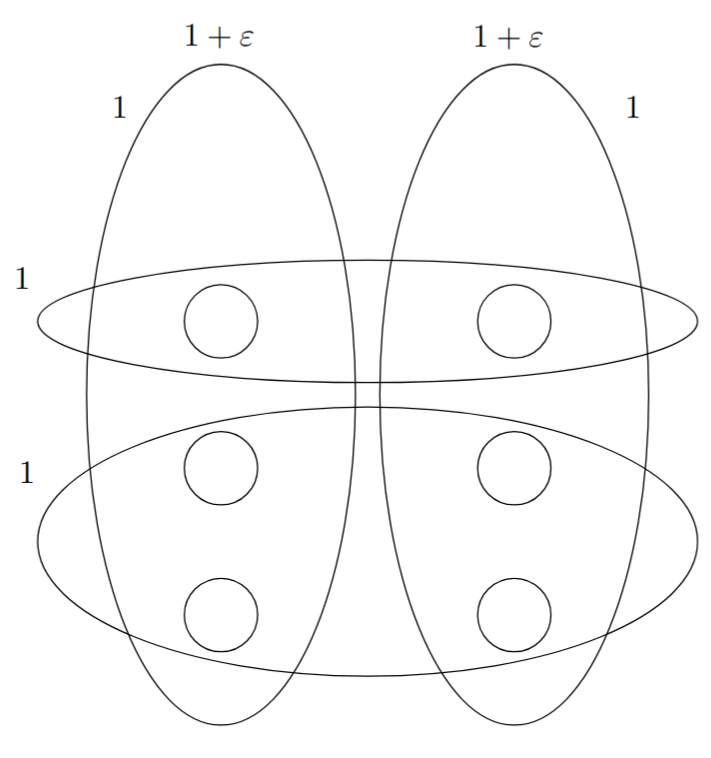
\includegraphics[width=0.5\columnwidth]{img/VertexCoverInput}
\end{center}

La soluzione ottima ovviamente è prendere i due insiemi più grandi per un costo di $2(1 + \epsilon)$.\\

\newpage

Ma GreedySetCover su questo input sceglierà per primo l'insieme che copre $n/2$ punti con costo $1$ in quanto 
$$ \frac{1}{n/2} < \frac{1+\epsilon}{n/2} $$

Al passaggio dopo i due insiemi grossi conterranno $n/4$ nuovi elementi e si ripeterà:
$$ \frac{1}{n/4} < \frac{1+\epsilon}{n/4} $$

Quindi non sceglierà mai i due insiemi grandi ma sempre le intersezioni che coprono sempre meno elementi. Di conseguenza:
$$ w = \log n $$
$$ w^\ast = 2 + 2 \epsilon$$
$$ \implies \frac{w}{w^\ast} = \frac{\log n}{2 + 2 \epsilon} = \Omega (\log n)$$

Quindi questo algoritmo fa le scelte peggiori possibili, ed è l'input peggiore possibile.\\

\paragraph{Fun fact:} Se $P \neq NP$ non esiste un algoritmo che approssimi SetCover meglio di $(1 - O(1)) \log n$. Questo pone SetCover nell'insieme dei problemi $\log n$-APX.\\

\newpage